\ifdefined\included
\else
\setcounter{chapter}{8} %% Numéro du chapitre précédent ;)
\dominitoc
\faketableofcontents
\fi

\chapter{The director task: Assessing cognitive architectures}
\chaptermark{The director task}
\minitoc

The contribution presented in this chapter is excerpted from our work, submitted to the RO-MAN 2021 conference. This contribution closes this thesis and has been achieved in collaboration with other PhD students of the HRI teams. Guilhem Buisan was concerned about the task planning part. Amandine Mayima worked on the supervision component. Kathleen Belhassein has designed the presented task with us giving her psychologist point of view to create a task on which user studies could be performed. The engineer Yannick Riou worked on the motion planning component allowing us to develop a task where the robot acts on its environment. My concern about this task has been the integration of my previous contributions about Ontology and the REG. It has also been the opportunity to create an entire architecture extending the ones presented all along with this thesis and linked with the contributions of the team. Finally, I contribute to the Situation assessment component and on the Language understanding part.

The components related to my teammates will be briefly described to give an overview of the architecture. The newly introduced capabilities on which I work will be more detailed to explain the links I make between all my contributions, centred on the knowledge representation.

\section{Introduction}

Developing robotic architectures adapted to Human-Robot Interaction and thus able to carry out interactions in an acceptable way is still today a real challenge. The complexity comes, among other things, from the number of capabilities which the robot must be endowed with and therefore from the number of software components which must be integrated in a coherent manner. Such architectures should provide the robot with the capability to perceive its environment and its partners, to merge and interpret this perceptual information, to communicate about it, to plan tasks with its partner, to estimate the others' perspective and mental state, etc. Once developed, evaluating these architectures can be difficult because all these components grouped into a single system. The tasks we usually want the robot to handle must highlight a maximum of abilities, while still being simple enough to be reproduced by the community. Moreover, we should be able to conduct user studies with it to validate choices regarding naive users.

Since a long term goal of the robotic field is to see robots evolving in our daily life, many tasks and scenarios have been inspired by everyday activities. Even if these tasks offer a large variety of situation to ba handle since the human partner is not limited in its actions, they have the disadvantage of not highlighting some subtle abilities which are nevertheless necessary for good interaction.
The robot guide task \cite{satake_2015_should} in mall, museum, or airport, requires high communication skills to understand free queries (possibly involving chatting) and respond to them, whether to indicate a direction or to give advice. However, the perception needs can be limited due to the vast environments, as well as the perspective-taking needs due to the same perception of the environment by the robot and the human\footnote{For sure we can find some tricky cases where it could help but they do not reflect common situations.}. Finally, with such a task the human partner is not an actor of the task and just has to listen to the robot once their question is asked. Even if being in more constrained environments, bartender-like tasks~\cite{petrick_2012_social} have the same disadvantages. Indeed, the human is considered as a customer, and as such, the interaction with the robot is limited. The robot will never ask the human to help it for performing a task and their actions do not require coordination either full collaboration.

To involve the human partner in the task and requiring him to act with the robot, assembly-like tasks~\cite{tellex_2014_asking} can be used. Nevertheless, in most cases, the human acts as an assistant rather than as a partner as full collaboration can be challenging to perform. The robot thus elaborates a plan and performs the assemble, then asks for help when detecting errors during the execution (e.g., when it cannot reach some pieces). Here the task leads to unidirectional communication. Moreover, because in such a task both the robot and the human have equivalent knowledge about the environment, it can be hard to design situations where belief divergence appear and thus perspective-taking would be required.

Scaling down an everyday task to transform it into a toy task around a table can deduce the task complexity and allow easy reproducibility. Moreover, it allows making the robot and the human work in the vicinity of each other, with smaller robots for example. With the toy version of the assembly task presented in~\cite{brawer_2018_situated}, the human is more involved in the task. They ask the robot to take pieces and to hold them to help them assemble a chair. Even if the communication is unidirectional, we could imagine inverting the roles to test different abilities. Moreover, communication implies objects referring with the use of various visual features about the entities. Even if both agents have the same knowledge about the environment, the communication is grounded according to the current state of the world. In this task, no decision has to be made by the robot but once again, inverting the roles could open other challenges.

To focus studies around perspective-taking and belief management, the Sally and Anne scenario, coming from a psychology test, has been studied in robotic~\cite{milliez_2014_framework}. In this scenario, the robot is a spectator of a situation where two humans come and go from a room, and move an object from a box to another. Since a human is in the room when the other is acting, a belief divergence appears between the two humans and the robot has to understand it. While the task highlights the belief management, it is first limited regarding the perspective-taking since the human presence or not could be sufficient to estimate the humans beliefs\footnote{When both humans are in the room they have the same perception of the scene but have different beliefs about hidden objects. Perspective-taking would be required if the humans could lean over the boxes to check what is inside.}. Moreover, the humans do not act with the robot since it is just a spectator of the scene. In addition, no goal is formulated and the human neither interacts with one another. Finally, no communication is needed in the task. The scenario is thus focussed on the analyse of a situation.

In this chapter, we first propose a new psychology-inspired task that we think to be challenging for the Human-Robot Interaction community and rich enough to be extended. Inter alia, it requires perspective-taking, planning, knowledge representation with theory of mind, manipulation, communication, and decision-making. Then, we present the robotic cognitive architecture that we develop to perform the task in its nominal cases. Finally, on the basis of the presented task and what has been developed, we present a discussion about the possible future challenges and evaluations for the research community, with possible extensions of the task.

\section{From psychology to Human-Robot Interaction}

\subsection{The original task}

\begin{figure}[ht!]
\centering
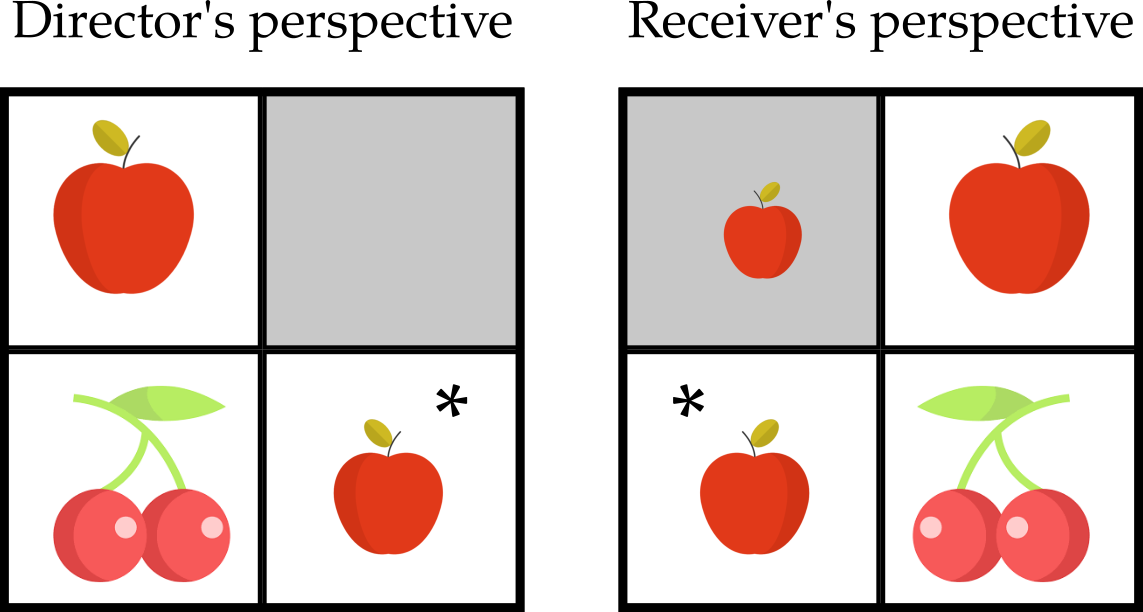
\includegraphics[scale=0.25]{figures/chapter9/dt_apple.png}
\caption{\label{fig:chap9_dt_apple} Sample display from the director's and the receiver's perspectives. The asterisk indicates the target object / competitor. Giving the sentence "the smallest apple" the receiver should find the good one even if he can see a smallest one in its perspective. }
\end{figure}

\subsection{The adapted task}

\begin{figure}[ht!]
\centering
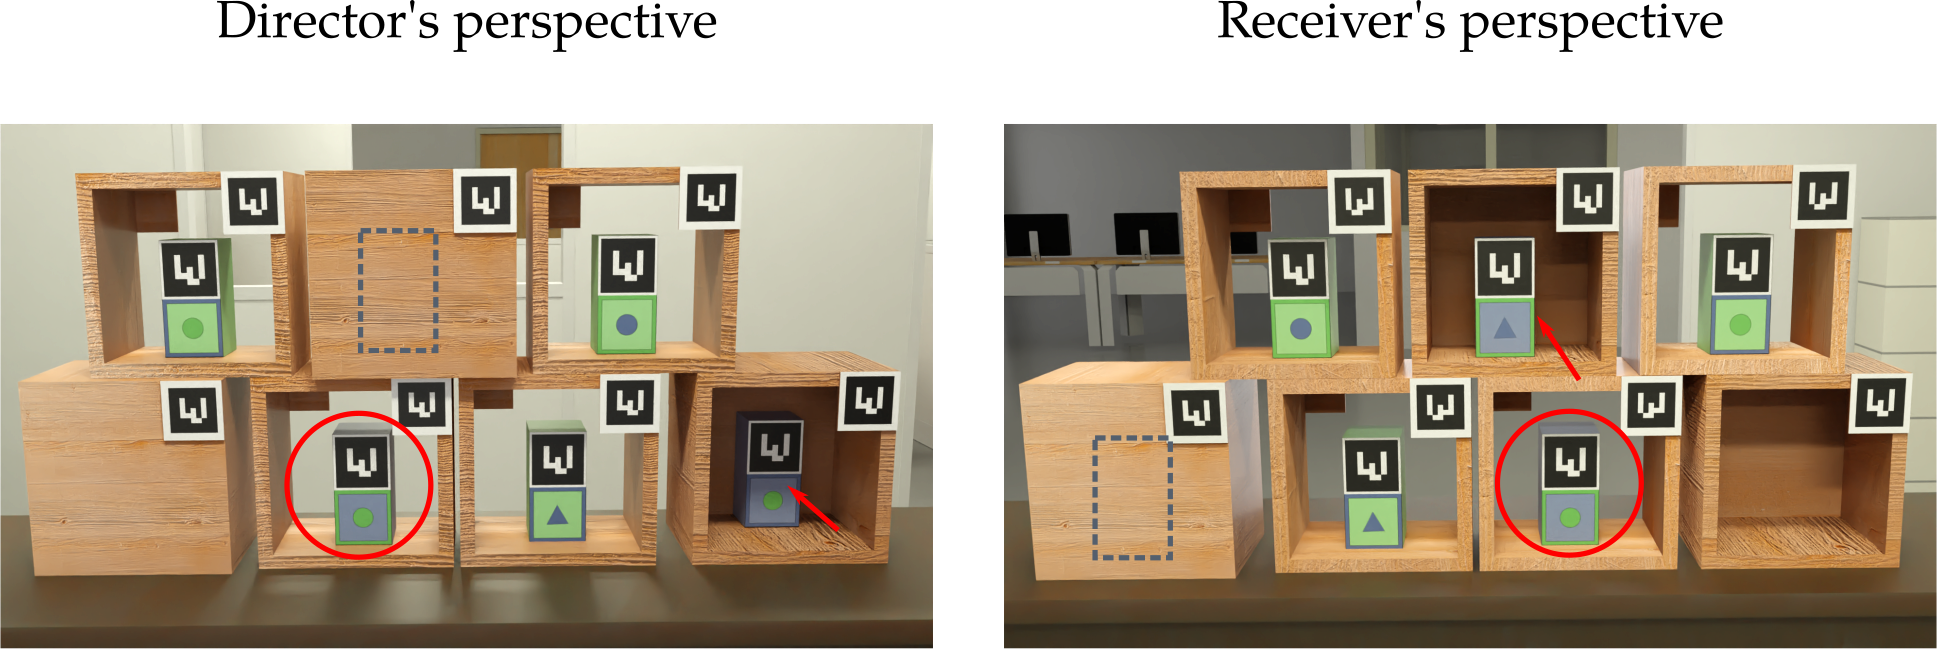
\includegraphics[width=\textwidth]{figures/chapter9/setup.png}
\caption{\label{fig:chap9_setup} A director task setup adapted to the HRI with the director's and receiver's perspectives. For the material, each element (blocks and compartment) is equipped with AR-tags allowing their detection by the robot. Each block has four visual characteristics: a main color, a border color, a geometric figure, and a figure color. Compartments can be hidden for the director or the receiver. For the director to designate the block marked with a red circle, estimating the receiver's perspective, he can refer to it by its main color (blue) because he estimates the other blue block is not visible by the receiver. For the receiver, by taking into account the director's perspective, he can understand the referred block as he estimates the other blue block to not be visible by the director.}
\end{figure}

\section{The cognitive architecture and the knowledge link}

\begin{figure}[ht!]
\centering
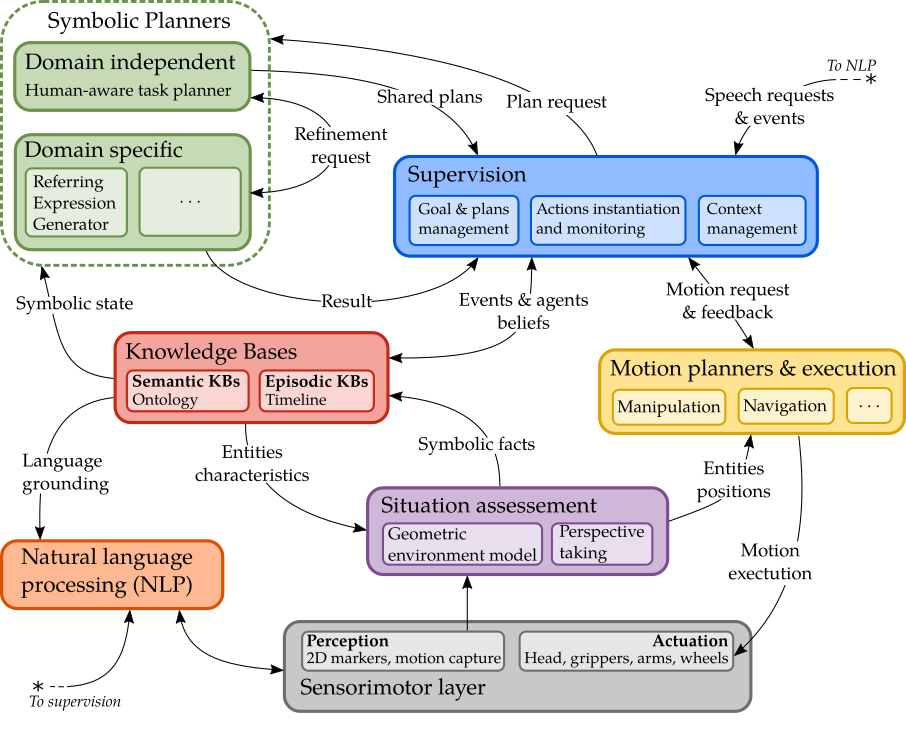
\includegraphics[width=\textwidth]{figures/chapter9/architecture.png}
\caption{\label{fig:chap9_architecture} An overview of the cognitive architecture developed to handle the Director Task. Each block does not necessarily represent one software component but rather an architectural module (in terms of the features it implements). The arrows represent the type of information exchanged between the modules. This architecture extends the ones presented all along with this thesis.}
\end{figure}

\subsection{The declarative memory}

\subsection{The Situation Assessment}

\begin{figure}[ht!]
\centering
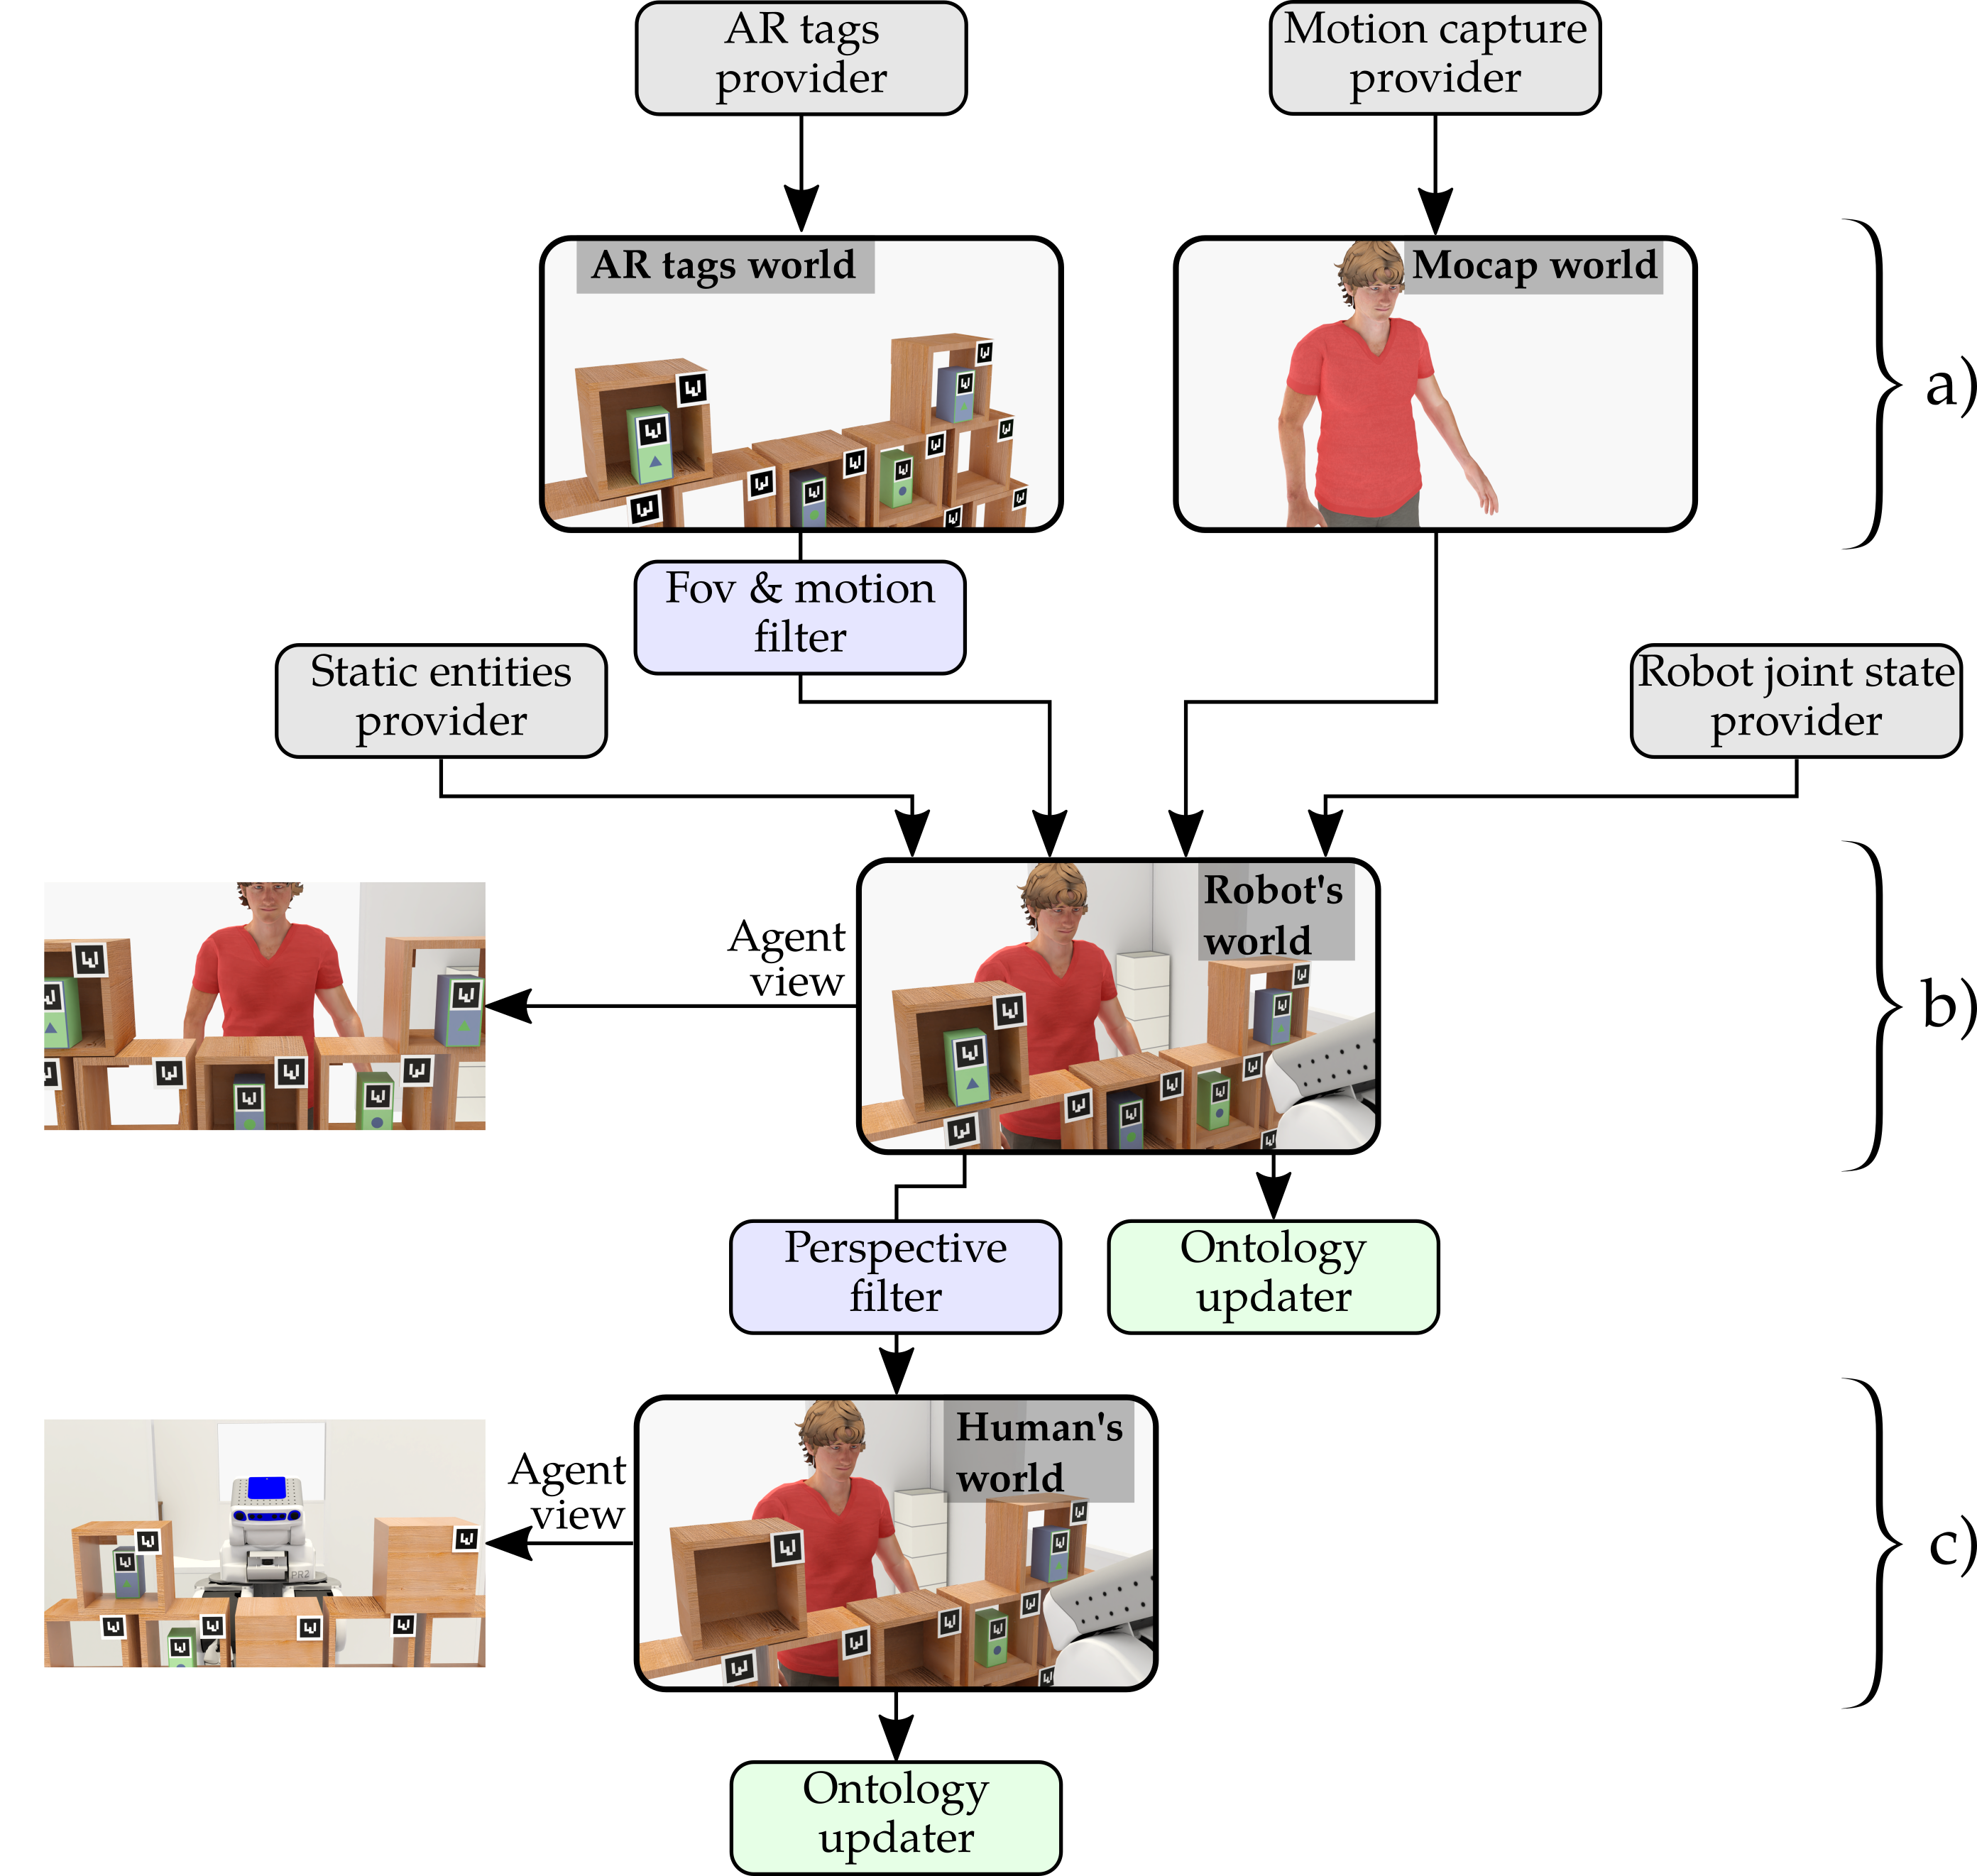
\includegraphics[width=\textwidth]{figures/chapter9/uwds/uwds.png}
\caption{\label{fig:chap9_uwds} The world cascading structure of the geometrical situation assessment system. The two worlds at the top (a) are build from the perception systems and filtered. The world of the middle (b) merges the different perception information and computes symbolic facts on it. The world at the bottom (c) is the estimation of the human world representation and is computed from perspective-taking in the robot's world. Like for the world of the middle, symbolic facts are computed and sent to the semantic knowledge base.}
\end{figure}

\subsection{The supervision}


\section{Integration on a robotic system}

\subsection{The integrated features}

\subsection{Future developments}